\PassOptionsToPackage{unicode=true}{hyperref} % options for packages loaded elsewhere
\PassOptionsToPackage{hyphens}{url}
%
\documentclass[11pt,ignorenonframetext,aspectratio=169]{beamer}
\usepackage{pgfpages}
\setbeamertemplate{caption}[numbered]
\setbeamertemplate{caption label separator}{: }
\setbeamercolor{caption name}{fg=normal text.fg}
\beamertemplatenavigationsymbolsempty
% Prevent slide breaks in the middle of a paragraph:
\widowpenalties 1 10000
\raggedbottom
\setbeamertemplate{part page}{
\centering
\begin{beamercolorbox}[sep=16pt,center]{part title}
  \usebeamerfont{part title}\insertpart\par
\end{beamercolorbox}
}
\setbeamertemplate{section page}{
\centering
\begin{beamercolorbox}[sep=12pt,center]{part title}
  \usebeamerfont{section title}\insertsection\par
\end{beamercolorbox}
}
\setbeamertemplate{subsection page}{
\centering
\begin{beamercolorbox}[sep=8pt,center]{part title}
  \usebeamerfont{subsection title}\insertsubsection\par
\end{beamercolorbox}
}
\AtBeginPart{
  \frame{\partpage}
}
\AtBeginSection{
  \ifbibliography
  \else
    \frame{\sectionpage}
  \fi
}
\AtBeginSubsection{
  \frame{\subsectionpage}
}
\usepackage{lmodern}
\usepackage{amssymb,amsmath}
\usepackage{ifxetex,ifluatex}
\usepackage{fixltx2e} % provides \textsubscript
\ifnum 0\ifxetex 1\fi\ifluatex 1\fi=0 % if pdftex
  \usepackage[T1]{fontenc}
  \usepackage[utf8]{inputenc}
  \usepackage{textcomp} % provides euro and other symbols
\else % if luatex or xelatex
  \usepackage{unicode-math}
  \defaultfontfeatures{Ligatures=TeX,Scale=MatchLowercase}
\fi
% use upquote if available, for straight quotes in verbatim environments
\IfFileExists{upquote.sty}{\usepackage{upquote}}{}
% use microtype if available
\IfFileExists{microtype.sty}{%
\usepackage[]{microtype}
\UseMicrotypeSet[protrusion]{basicmath} % disable protrusion for tt fonts
}{}
\IfFileExists{parskip.sty}{%
\usepackage{parskip}
}{% else
\setlength{\parindent}{0pt}
\setlength{\parskip}{6pt plus 2pt minus 1pt}
}
\usepackage{hyperref}
\hypersetup{
            pdftitle={CS5014 Machine Learning},
            pdfauthor={Lei Fang},
            pdfborder={0 0 0},
            breaklinks=true}
\urlstyle{same}  % don't use monospace font for urls
\newif\ifbibliography
\setlength{\emergencystretch}{3em}  % prevent overfull lines
\providecommand{\tightlist}{%
  \setlength{\itemsep}{0pt}\setlength{\parskip}{0pt}}
\setcounter{secnumdepth}{0}

% set default figure placement to htbp
\makeatletter
\def\fps@figure{htbp}
\makeatother

%\usepackage[latin1]{inputenc}

\usepackage{graphicx}
\usepackage{rotating}
%\setbeamertemplate{caption}[numbered]
\usepackage{hyperref}
\usepackage{caption}
\usepackage[normalem]{ulem}
%\mode<presentation>
\usepackage{wasysym}
\usepackage{amsmath}
\usepackage{mathtools}
\usepackage[skins,theorems]{tcolorbox}
% \usepackage[,dvipsnames]{xcolor}
\tcbset{highlight math style={enhanced,
  colframe=red,colback=white,arc=0pt,boxrule=1pt}}
  
\usepackage{subfig}
% \usefonttheme{professionalfonts}
% \usepackage{times}
\usepackage{tikz}
\usepackage{amsmath}
\usepackage{verbatim}
\usetikzlibrary{arrows,shapes}
  

\newcommand{\normal}[2]{\ensuremath{\mathcal{N}\left (#1,#2 \right )}}
\newcommand{\Gaussian}[3]{\ensuremath{\frac{1}{\sqrt{2\pi}#3}
\text{exp}\left \{-\frac{1}{2#3^2} (#1-#2)^2 \right \}}}
\newcommand{\argmax}{\operatornamewithlimits{argmax}}
\newcommand{\expo}[1]{\ensuremath{\text{exp}\left \{ #1 \right \}}}
\newcommand{\studentt}[4]{\ensuremath{\mathcal{T}_{#4}(#1,#2,#3)}}
\newcommand{\vv}[1]{\boldsymbol{#1}}
\newcommand{\Prb}{\ensuremath{\mathbb{P}}}
\newcommand{\studenttk}[4]{\ensuremath{\mathcal{T}_{#4}(#1,#2,#3)}}
\newcommand{\argmin}{\operatornamewithlimits{argmin}}
\newcommand{\NIG}{\mathcal{NIG}}
\newcommand{\N}{\mathcal{N}}
\newcommand{\T}{\mathcal{T}}
\newcommand{\IG}{\mathcal{IG}}
\newcommand{\IW}{\mathcal{IW}}
\newcommand{\NNIW}{\mathcal{NNIW}}
\newcommand{\vct}{\text{vec}}
\newcommand{\NN}{\mathcal{NN}}
\newcommand{\tr}{\text{tr}}
\newcommand{\di}[2]{\ensuremath{ #1^{(#2)}}}
\newcommand{\dd}[1]{\ensuremath{ #1^{(i)}}}
\newcommand{\Di}[2]{\ensuremath{ \vv{#1}^{(#2)}}}

\newcommand{\E}[1]{\ensuremath{\mathbb{E}[#1]}}
\newcommand{\Var}[1]{\mathrm{Var}[#1]}
\newcommand{\Cov}[2]{\mathrm{Cov}[#1,#2]}
\newcommand{\Cor}[2]{\mathrm{Cor}[#1,#2]}

\usepackage[]{algorithm2e}
% \setbeamertemplate{navigation symbols}{}
\usepackage{tcolorbox}


%\titlegraphic{\includegraphics[width=0.3\paperwidth]{\string~/Dropbox/teaching/clemson-academic.png}}
\titlegraphic{\includegraphics[width=0.1\paperwidth]{./figs/crest.pdf}}
\setbeamertemplate{title page}[empty]

\setbeamerfont{subtitle}{size=\small}
\setbeamerfont{normal text}{size=\tiny}
\setbeamercovered{invisible}

\definecolor{clemsonpurple}{HTML}{522D80}
\definecolor{stablue}{HTML}{0052cc}
\definecolor{stared}{HTML}{ff4d4d}
\definecolor{clemsonorange}{HTML}{F66733}
\newcommand{\empha}[1]{\textbf{\textcolor{stablue}{#1}}}
\setbeamercolor{frametitle}{fg=stablue,bg=white}
\setbeamercolor{title}{fg=stablue,bg=white}
\setbeamercolor{local structure}{fg=stablue}
\setbeamercolor{section in toc}{fg=stablue,bg=white}
\setbeamercolor{subsection in toc}{fg=stared,bg=white}
\setbeamercolor{item projected}{fg=stablue,bg=white}
\setbeamertemplate{itemize item}{\color{stablue}$\bullet$}
\setbeamertemplate{itemize subitem}{\color{stablue}\scriptsize{$\bullet$}}
\let\Tiny=\tiny

%\makeatletter
%\setbeamertemplate{footline}{%
%\leavevmode
%\vbox{\begin{beamercolorbox}[dp=1.25ex,ht=2.75ex]{fg=black}%
%  \hspace*{1em}\insertsectionhead%
%  \ifx\insertsubsectionhead\@empty\relax\else$\quad\mid\quad$\insertsubsectionhead\fi :
%  \end{beamercolorbox}%
%  }%
%}
%\makeatother

\setbeamercolor{footercl}{fg=white,bg=stablue}
\setbeamerfont{stafont}{size = \large}
\setbeamerfont{footerfont}{size = \tiny}
% \makeatother
% \setbeamertemplate{footline}
% {
%   \leavevmode%
%   \hbox{%
%   \begin{beamercolorbox}[wd=.5\paperwidth,ht=5ex,dp=1ex, left]{footercl}%
%     \usebeamerfont*{stafont}\hspace*{1ex}\insertshortinstitute
%   \end{beamercolorbox}%
%   \begin{beamercolorbox}[wd=.25\paperwidth,ht=5ex,dp=1ex,center]{footercl}%
%     \usebeamerfont*{footerfont}\insertshorttitle\hspace*{1ex} \insertframenumber{}
%   \end{beamercolorbox}%
%   \begin{beamercolorbox}[wd=.25\paperwidth,ht=5ex,dp=1ex,right]{footercl}%
%    \includegraphics[height=5ex]{stalogo.png}
%   \end{beamercolorbox}}%
%   \vskip0pt%
% }
% \makeatletter
\makeatletter
\setbeamertemplate{footline}
{
  \leavevmode%
  \hbox{%
  \fontsize{13}{13}\fontfamily{ppl}\selectfont
  \begin{beamercolorbox}[wd=.5\paperwidth,ht=2.25ex,dp=1ex,left]{footercl}%
    \usebeamerfont{author in head/foot}\hspace*{1ex}\insertshortinstitute
   \end{beamercolorbox}%
   \begin{beamercolorbox}[wd=.25\paperwidth,ht=2.25ex,dp=1ex,right]{footercl}%
    % \hfill\hfill\hfill\hfill\hfill\hfill\hfill\hfill\hfill\hfill
    \parbox{.25\paperwidth}{\fontfamily{cmss}\selectfont{\hfill\hfill \usebeamerfont{footerfont}\insertshorttitle~\insertframenumber{}}}
  \end{beamercolorbox}%
  \begin{beamercolorbox}[wd=.25\paperwidth,ht=2.25ex,dp=1ex,left]{footercl}%
    \parbox{.25\paperwidth}{\hfill\includegraphics[height=1cm]{./figs/stalogo.png}}% original: 2ex
  \end{beamercolorbox}}%
  \vskip0pt%
}
\makeatother

\setbeamertemplate{navigation symbols}{}

% \AtBeginDocument{\author[L. Fang]{Lei Fang} \institute[www.st-andrews.ac.uk]{School of Computer Science, University of St Andrews}}

% \newcommand{\Ffootline}{%                   %%defines a new command called \Ffootline
% %\insertshortauthor,                         %%puts the abbreviated form of the author's name in the left corner
% \insertshorttitle,
% \insertshortinstitute, 
% \insertshortdate %%puts the abbreviated form of the author's institution in the middle
% \hfill
% \insertsection,
% \insertframenumber/\inserttotalframenumber} %%includes the current slide number over the total slide number in the right corner
% \setbeamertemplate{footline}{%              %%sets the options for the footline
% \usebeamerfont{structure}                   %%uses the same fonts adopted for the structure of the presentation 
% \Tiny\hspace*{4mm} \Ffootline \hspace{4mm}  %%sets the size of the font to Tiny and includes the content of the \Ffootline
% }                                           %%command leaving a margin of 4mm to the right and left of the content.



\AtBeginPart{}
\AtBeginSection{}
\AtBeginSubsection{}
\AtBeginSubsubsection{}
\setlength{\emergencystretch}{0em}
\setlength{\parskip}{0pt}
\AtBeginDocument{\author[L. Fang]{Lei Fang} \title[L13 Unsupervised Learning]{CS5014 Machine Learning}\institute[www.st-andrews.ac.uk]{School of Computer Science, University of St Andrews}}
\newenvironment{cols}[1][]{}{}

\newenvironment{col}[1]{\begin{minipage}{#1}\ignorespaces}{%
\end{minipage}
\ifhmode\unskip\fi
\aftergroup\useignorespacesandallpars}

\def\useignorespacesandallpars#1\ignorespaces\fi{%
#1\fi\ignorespacesandallpars}

\makeatletter
\def\ignorespacesandallpars{%
  \@ifnextchar\par
    {\expandafter\ignorespacesandallpars\@gobble}%
    {}%
}
\makeatother

\title{CS5014 Machine Learning}
\providecommand{\subtitle}[1]{}
\subtitle{Lecture 13 Unsupervised Learning}
\author{Lei Fang}
\date{Spring 2021}

\begin{document}
\frame{\titlepage}

\begin{frame}{Some responses: geometry of ridge regression}
\protect\hypertarget{some-responses-geometry-of-ridge-regression}{}

\begin{cols}

\begin{col}{0.30\textwidth}

\begin{center}\includegraphics[width=1\linewidth]{lecture13_files/figure-beamer/unnamed-chunk-1-1} \end{center}

\end{col}

\begin{col}{0.70\textwidth}

\[\vv{\beta}_{\text{ridge}} \equiv \argmin_{\vv{\beta}} \underbrace{||\vv{y}-\vv{X\beta}||_2^2}_{L(\vv{\theta})} + \lambda ||\vv{\beta}||_2^2\]
\[\vv{\beta}_{\text{ridge}} = (\vv{X}^T\vv{X} + \lambda \vv{I})^{-1}\vv{Xy}\]

\begin{itemize}
\tightlist
\item
  assume feature vectors of \(\vv{X}\) are norm 1 and orthogonal
  i.e.~orthogonormal: \(\vv{X}^T\vv{X} = \vv{I}\)
\end{itemize}

\[\footnotesize \vv{\beta}_{\text{ridge}} = \frac{1}{1+\lambda} (\vv{X}^T\vv{X})^{-1}\vv{Xy}= \frac{1}{1+\lambda}\vv{\beta}_{ML}\]

\begin{itemize}
\tightlist
\item
  why the likelihood (red) contours are circular for this case ?
  \pause remember the Hessian of \(L(\vv{\theta})\)?
  \[\footnotesize H_{L} = 2\vv{X}^T\vv{X}\propto \vv{I}\]
\item
  uniform discount: \(\beta_k\) receives the same discount:
  \(\frac{1}{1+\lambda}\)
\end{itemize}

\end{col}

\end{cols}

\end{frame}

\begin{frame}{Some responses: some other cases}
\protect\hypertarget{some-responses-some-other-cases}{}

\begin{cols}

\begin{col}{0.30\textwidth}

\begin{center}\includegraphics[width=1\linewidth]{lecture13_files/figure-beamer/unnamed-chunk-2-1} \end{center}

\end{col}

\begin{col}{0.7\textwidth}

When \(H_L \neq \vv{I}\) , the shrinkage is \textbf{NOT} uniform;

\[{\beta}^{\text{ridge}}_k = \frac{\sigma_k}{{\sigma_k}+\lambda} {\beta}^{ML}_k\;\;\;\]

\begin{itemize}
\tightlist
\item
  \(\sigma_k\) is the directional curvature of \(\vv{X}^T\vv{X}\) (also
  the eigen value)
\item
  flat curve (\(\beta_1\) direction) \(\Rightarrow\) \(\sigma_k\)
  smaller \(\Rightarrow\) more discount
\item
  curvy curve (\(\beta_2\) direction) \(\Rightarrow\) \(\sigma_k\)
  larger \(\Rightarrow\) less discount
\item
  makes perfect sense!

  \begin{itemize}
  \tightlist
  \item
    flat means less confident (or large variance): shrink more
  \item
    peak means confident estimate (small variance): shrink less
  \end{itemize}
\end{itemize}

\footnotesize \((*)\) the equation is true when \(\vv{X}^T\vv{X}\) is a
diagonal matrix; up to basis translation for more general cases

\end{col}

\end{cols}

\end{frame}

\begin{frame}{Today's topic}
\protect\hypertarget{todays-topic}{}

Unsupervised learning

\begin{itemize}
\tightlist
\item
  clustering
\item
  k-means
\end{itemize}

Revisit multivariate Gaussian

Revisit k-means

\begin{itemize}
\tightlist
\item
  mixture of Gaussians
\item
  EM algorithm for mixture model

  \begin{itemize}
  \tightlist
  \item
    K-means is just a specific case
  \end{itemize}
\item
  other kinds of mixture models
\end{itemize}

\end{frame}

\begin{frame}{Unsupervised learning}
\protect\hypertarget{unsupervised-learning}{}

\end{frame}

\begin{frame}{Clustering}
\protect\hypertarget{clustering}{}

\end{frame}

\begin{frame}{K-means}
\protect\hypertarget{k-means}{}

\end{frame}

\begin{frame}{K-means}
\protect\hypertarget{k-means-1}{}

\end{frame}

\begin{frame}{Demonstration}
\protect\hypertarget{demonstration}{}

\end{frame}

\begin{frame}{Limitations of K-means}
\protect\hypertarget{limitations-of-k-means}{}

\end{frame}

\begin{frame}{Dissect multivariate Gaussians}
\protect\hypertarget{dissect-multivariate-gaussians}{}


\tikzstyle{every picture}+=[remember picture]
\everymath{\displaystyle}
\tikzstyle{na} = [baseline=-.5ex]

\begin{equation*}
p(\vv{x})={N}(\vv{x}; \vv{\mu}, \vv{\Sigma}) \equiv \tikz[baseline]{  \node[fill=blue!20,anchor=base] (t1) {$\frac{1}{(2\pi)^{d/2} |\vv{\Sigma}|^{1/2}}$};}
\tikz[baseline] {\node[fill=purple!10, circle, anchor=base] (t2) {$\exp$}; }   [\tikz[baseline] {\node[fill=green!80!black, anchor=base] (t3){$-$};}\frac{1}{2} 
\underbrace{\tikz[baseline]{\node[fill=red!20, anchor=base] (t4) {$(\vv{x} -\vv{\mu})^T\vv{\Sigma}^{-1}(\vv{x}-\vv{\mu})$};} }_{d_{\vv{\Sigma}}}
 ]
\end{equation*}


\begin{columns}
\begin{column}{0.7\textwidth}\footnotesize
\begin{itemize}[<+->]
    \item \textcolor{red!80}{a distance measure \tikz\node [coordinate] (qf) {};}:(aka mahalanobis distance) $$d_{\vv{\Sigma}}(\vv{x};\vv{\mu}): \text{between }\vv{x}\text{ and } \vv{\mu}$$
    \item \textcolor{green!80!black}{$-$}\tikz\node [coordinate] (neg) {};: $p$ is \textcolor{green!80!black}{\textbf{negatively}} related to the distance
        $$\text{larger } d_{\vv{\Sigma}}(\vv{x};\vv{\mu} ) \Rightarrow \text{further away }\vv{x} \text{ from } \vv{\mu} \Rightarrow  \text{smaller } p$$
    \item \textcolor{purple!80}{$\exp$}: \tikz\node [coordinate] (exp) {}; makes sure $p(\vv{x})>0$
       
    \item \textcolor{blue!80}{normalising\tikz\node [coordinate] (n3) {}; constant}: s.t. $\int N(\vv{x};\cdot, \cdot) d\vv{x} = 1$; $$|\vv{\Sigma}|: \text{ determinant; a volume measure-ish quantity}$$
\end{itemize}


\begin{tikzpicture}[overlay]
        \path[->]<1-> (qf) edge [bend left, red!80] (t4);
        \path[->]<2-> (neg) edge [bend right, green!80!black] (t3);
        \path[->]<3-> (exp) edge [bend right, purple!80!black] (t2);
        \path[->]<4-> (n3) edge [bend right, blue!80] (t1);
\end{tikzpicture}
\end{column}
\begin{column}{0.35\textwidth}
\begin{figure}
    \centering
    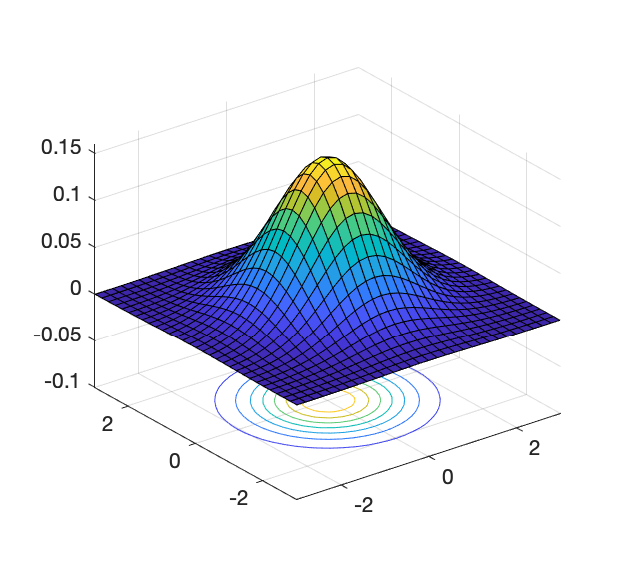
\includegraphics[width = 1\textwidth]{./figs/2dMVN1}
 % \caption{}
\end{figure}  
\end{column}
\end{columns}

\end{frame}

\begin{frame}{Dissect multivariate Gaussians}
\protect\hypertarget{dissect-multivariate-gaussians-1}{}

\textbf{Key message}: \(d_{\Sigma}\) (the distance) determines equal
\(p(\vv{x})\) levels

\begin{equation*}\footnotesize
p(\vv{x}) \equiv \underbrace{\tikz[baseline]{  \node[fill=blue!20,anchor=base] (t1) {$\frac{1}{(2\pi)^{d/2} |\vv{\Sigma}|^{1/2}}$};}}_{C: \text{normalising cst.}}
\overbrace{\tikz[baseline] {\node[fill=purple!10, circle, anchor=base] (t2) {$\exp$}; }   [\overbrace{\tikz[baseline] {\node[fill=green!50, anchor=base] (t3){$-$};}\frac{1}{2} 
\underbrace{\tikz[baseline]{\node[fill=red!20, anchor=base] (t4) {$(\vv{x} -\vv{\mu})^T\vv{\Sigma}^{-1}(\vv{x}-\vv{\mu})$};}}_{f_1=d_{\vv{\Sigma}}(\vv{x};\vv{\mu})}}^{f_2}
 ]}^{f_3}
\end{equation*}

\begin{cols}

\begin{col}{0.25\textwidth}

\begin{center}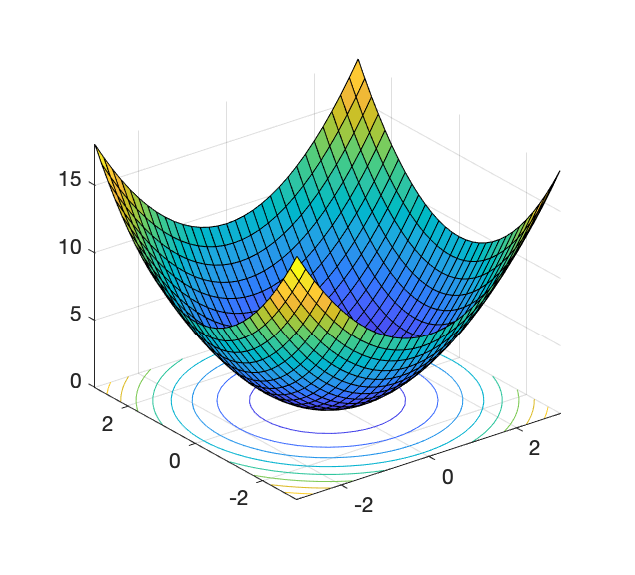
\includegraphics[height=0.3\textheight]{./figs/2dMVNQF0} \end{center}

\footnotesize

\begin{enumerate}
\tightlist
\item
  a distance measure: \(f_1(\vv{x})=d_{\vv{\Sigma}}(\vv{x};\vv{\mu})\)
\end{enumerate}

\end{col}

\begin{col}{0.25\textwidth}

\begin{center}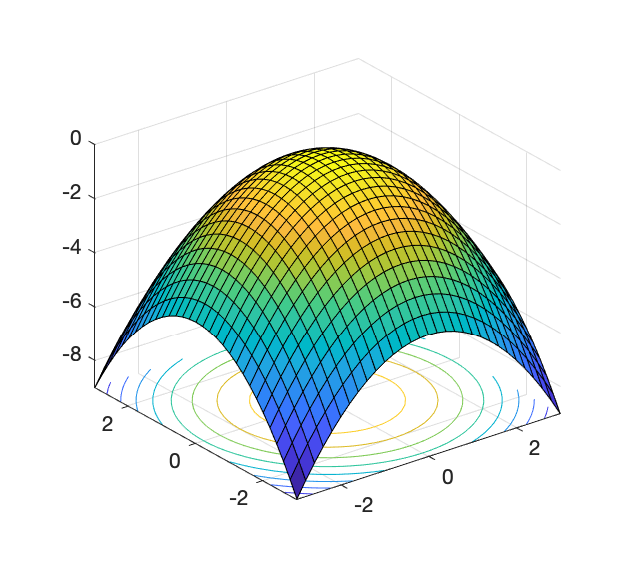
\includegraphics[height=0.3\textheight]{./figs/2dnegMVNQF0} \end{center}
\footnotesize

\begin{enumerate}
\setcounter{enumi}{1}
\tightlist
\item
  negated distance: \(f_2(\vv{x})=-\frac{1}{2}f_1(\vv{x})\) 
\end{enumerate}

\end{col}

\begin{col}{0.25\textwidth}

\begin{center}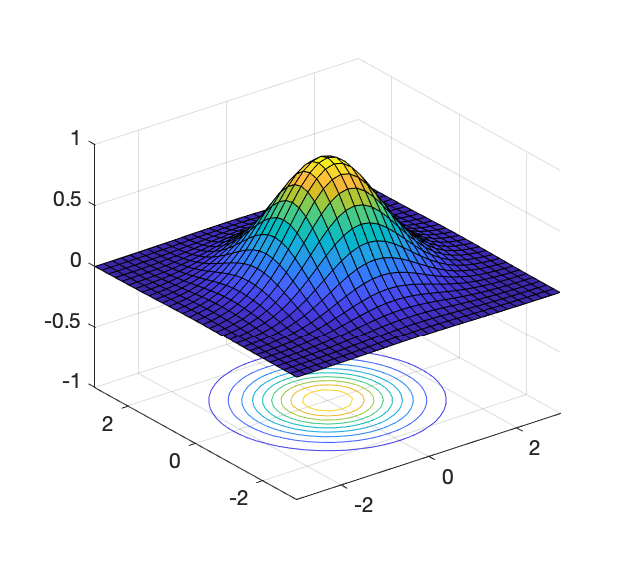
\includegraphics[height=0.3\textheight]{./figs/2dExpNegMVNQF0} \end{center}
\footnotesize

\begin{enumerate}
\setcounter{enumi}{2}
\tightlist
\item
  exp. to make sure \(p>0\): \(f_3(\vv{x})=e^{f_2(\vv{x})}\)
\end{enumerate}

\end{col}

\begin{col}{0.25\textwidth}

\begin{center}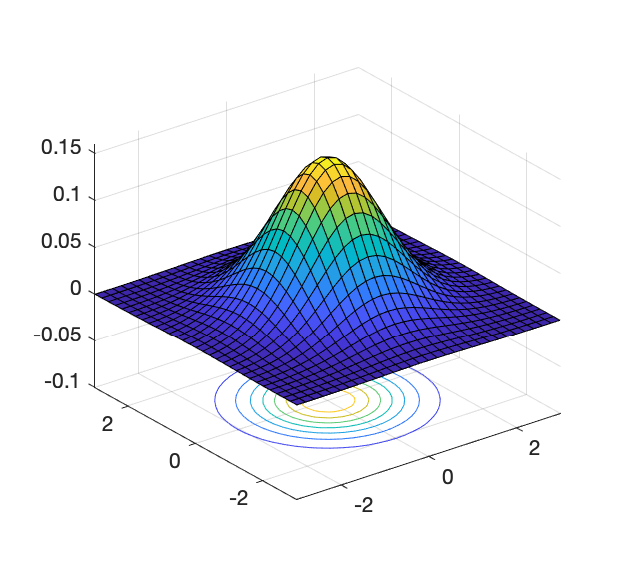
\includegraphics[height=0.3\textheight]{./figs/2dMVN1} \end{center}
\footnotesize

\begin{enumerate}
\setcounter{enumi}{3}
\tightlist
\item
  scaled to make sure \(\int p(\vv{x})d\vv{x}=1\):
  \(p(\vv{x})= C\cdot f_3(\vv{x})\)
\end{enumerate}

\end{col}

\end{cols}

\end{frame}

\begin{frame}{Covariance matrix and distance}
\protect\hypertarget{covariance-matrix-and-distance}{}

\[\vv{\Sigma}: \text{ variance-covariance matrix}\]

\begin{itemize}
\tightlist
\item
  \(d\times d\) symmetric matrix: \[\vv{\Sigma}= \vv{\Sigma}^T\]
\item
  positive definite (P.D.):
  \[\vv{v}^T\vv{\Sigma} \vv{v} >0,\;\;\; \forall \vv{v} \in R^d\]
\item
  why P.D. ? distance has to be positive ! (similar to univariate
  Gaussian: \((x-\mu)^2\cdot\sigma^{-2}>0\))
  \[(\vv{x}-\vv{\mu})^T \vv{\Sigma}^{-1} (\vv{x}-\vv{\mu}) >0, \;\;\;\text{where } \vv{v} = \vv{x}-\vv{\mu}\]

  \begin{itemize}
  \tightlist
  \item
    if \(\vv{\Sigma}\) is P.D., then \(\vv{\Sigma}^{-1}\) is also P.D.;
    so the above is a valid distance metric
  \end{itemize}
\end{itemize}

\footnotesize

Proof: Let \(\vv{y} = \vv{\Sigma}\vv{v}\); then
\(\vv{y}^T\vv{\Sigma}^{-1}\vv{y} = \vv{v}^T\vv{\Sigma}^T\vv{\Sigma}^{-1}\vv{\Sigma}\vv{v} = \vv{v}^T\vv{\Sigma}^T\vv{v} =\vv{v}^T\vv{\Sigma}\vv{v}> 0\)

\end{frame}

\begin{frame}{Diagonal \(\vv{\Sigma}\): implies independence}
\protect\hypertarget{diagonal-vvsigma-implies-independence}{}

If
\[\footnotesize \vv{\Sigma} = \begin{bmatrix}\sigma_1^2 & 0 & \ldots & 0 \\ 0 &\sigma^2_2 & \ldots & 0 \\ \vdots & \vdots & \ddots & \vdots \\ 0 & 0 & \ldots & \sigma^2_d  \end{bmatrix};\;\;\;\vv{\Sigma}^{-1} = \begin{bmatrix}\frac{1}{\sigma_1^2} & 0 & \ldots & 0 \\ 0 &\frac{1}{\sigma^2_2} & \ldots & 0 \\ \vdots & \vdots & \ddots & \vdots \\ 0 & 0 & \ldots & \frac{1}{\sigma^2_d}  \end{bmatrix}\]
Then \footnotesize 
\begin{align*} p(\vv{x}) &=  \frac{1}{(2\pi)^{d/2} |\vv{\Sigma}|^{1/2}} \exp\{-\frac{1}{2}
(\vv{x} -\vv{\mu})^T\vv{\Sigma}^{-1}(\vv{x}-\vv{\mu})\} =\frac{1}{(2\pi)^{d/2} (\prod_{i=1}^d \sigma_i^2)^{1/2}} \exp \{-\frac{1}{2} \sum_{i=1}^d (x_i-\mu_i)^2/\sigma_i^2\} \\
&= \prod_{i=1}^d \underbrace{\frac{1}{(2\pi)^{1/2} \sigma_i} \exp \{-\frac{1}{2} (x_i-\mu_i)^2/\sigma_i^2 \}}_{\text{unvariate Gaussian}} =\underbrace{ \prod_{i=1}^d p(x_i)}_{
\text{independence !}}
\end{align*}

and each \(p(x_i) = N(x_i; \mu_i, \sigma^2_i)\) is a univariate Gaussian

Remember independence ?
\colorbox{red!20}{it means knowing one does not inform the other: $p(x_i|\vv{x}_{/i})=p(x_i)$}

\end{frame}

\begin{frame}{Diagonal \(\vv{\Sigma}\): axis aligned ellipses}
\protect\hypertarget{diagonal-vvsigma-axis-aligned-ellipses}{}

\[\vv{\Sigma} = \begin{bmatrix}\sigma_1^2 & 0 \\ 0 & \sigma_2^2 \end{bmatrix};\vv{\Sigma}^{-1} = \begin{bmatrix}\frac{1}{\sigma_1^2} & 0 \\ 0 & \frac{1}{\sigma_2^2} \end{bmatrix}\;\;\; \text{so }d_{\vv{\Sigma}}(\vv{x}; \vv{0}) \text{ are axis aligned ellipses}\]

\begin{cols}

\begin{col}{0.25\textwidth}

\begin{center}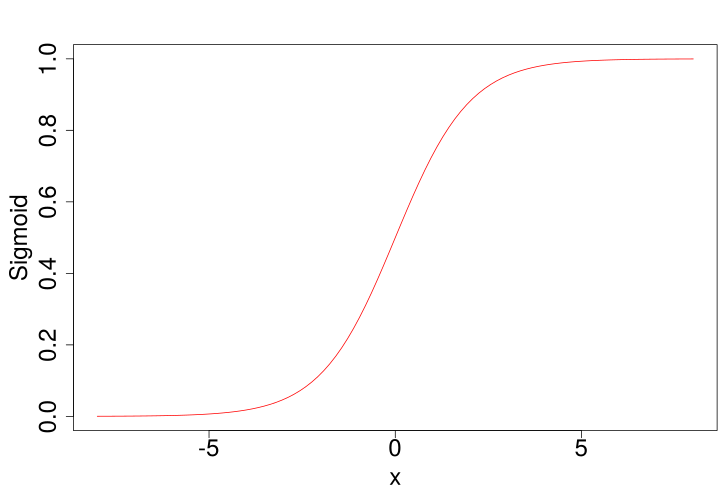
\includegraphics[width=0.9\linewidth]{lecture13_files/figure-beamer/unnamed-chunk-7-1} \end{center}

\[\vv{\Sigma} = \begin{bmatrix}1 & 0 \\ 0 & 1 \end{bmatrix}\]

\end{col}

\begin{col}{0.25\textwidth}

\begin{center}\includegraphics[width=0.9\linewidth]{lecture13_files/figure-beamer/unnamed-chunk-8-1} \end{center}

\[\vv{\Sigma} = \begin{bmatrix}3 & 0 \\ 0 & 3 \end{bmatrix}\]

\end{col}

\begin{col}{0.25\textwidth}

\begin{center}\includegraphics[width=0.9\linewidth]{lecture13_files/figure-beamer/unnamed-chunk-9-1} \end{center}

\[\vv{\Sigma} = \begin{bmatrix}1 & 0 \\ 0 & 2 \end{bmatrix}\]

\end{col}

\begin{col}{0.25\textwidth}

\begin{center}\includegraphics[width=0.9\linewidth]{lecture13_files/figure-beamer/unnamed-chunk-10-1} \end{center}

\[\vv{\Sigma} = \begin{bmatrix}2 & 0 \\ 0 & 1 \end{bmatrix}\]

\end{col}

\end{cols}

\end{frame}

\begin{frame}{General \(\vv{\Sigma}\): rotated ellipses}
\protect\hypertarget{general-vvsigma-rotated-ellipses}{}

\[\vv{\Sigma} = \begin{bmatrix}\sigma_1^2 & \sigma_{12} \\ \sigma_{21} & \sigma_2^2 \end{bmatrix}\;\;\; \text{ }d_{\vv{\Sigma}}(\vv{x}; \vv{0}) \text{ are rotated ellipses}\]

\begin{cols}

\begin{col}{0.25\textwidth}

\begin{center}\includegraphics[width=0.9\linewidth]{lecture13_files/figure-beamer/unnamed-chunk-11-1} \end{center}

\[\vv{\Sigma} = \begin{bmatrix}1 & 0.4 \\ 0.4 & 1 \end{bmatrix}\]

\end{col}

\begin{col}{0.25\textwidth}

\begin{center}\includegraphics[width=0.9\linewidth]{lecture13_files/figure-beamer/unnamed-chunk-12-1} \end{center}

\[\vv{\Sigma} = \begin{bmatrix}1 & 0.9 \\ 0.9 & 1 \end{bmatrix}\]

\end{col}

\begin{col}{0.25\textwidth}

\begin{center}\includegraphics[width=0.9\linewidth]{lecture13_files/figure-beamer/unnamed-chunk-13-1} \end{center}

\[\vv{\Sigma} = \begin{bmatrix}1 & -0.4 \\ -0.4 & 1 \end{bmatrix}\]

\end{col}

\begin{col}{0.25\textwidth}

\begin{center}\includegraphics[width=0.9\linewidth]{lecture13_files/figure-beamer/unnamed-chunk-14-1} \end{center}

\[\vv{\Sigma} = \begin{bmatrix}1 & -0.9 \\ -0.9 & 1 \end{bmatrix}\]

\end{col}

\end{cols}

\end{frame}

\begin{frame}{MLE of multivariate Gaussian}
\protect\hypertarget{mle-of-multivariate-gaussian}{}

Given \(\{\Di{x}{1}, \Di{x}{2}, \ldots, \Di{x}{m}\}\), assume
\(\Di{x}{i} \sim N(\vv{\mu},\vv{\Sigma})\); the goal is to estimate

\[\footnotesize \vv{\mu},\; \vv{\Sigma}\]

The log likelihood is:

\[\footnotesize \mathcal{L}(\vv{\mu}, \vv{\Sigma}) =  \log P(\{\Di{x}{i}\}_1^m|\vv{\mu}, \vv{\Sigma}) = \sum_{i=1}^m \log N(\Di{x}{i}; \vv{\mu}, \vv{\Sigma})\]

The MLE is defined as usual:

\[\footnotesize \vv{\mu}_{ML},\vv{\Sigma}_{ML} = \argmax_{\vv{\mu}, \vv{\Sigma}} \mathcal{L}(\vv{\mu}, \vv{\Sigma})\]

Take derivative and set to zero; after some tedious steps, the solution
is:

\begin{equation*}
\tikz[baseline]{  \node[fill=blue!20,anchor=base] (t1) {$\vv{\mu}_{ML} = \frac{1}{m} \sum_{i=1}^m \Di{x}{i},\;\;\; \vv{\Sigma}_{ML}= \frac{1}{m} \sum_{i=1}^m (\Di{x}{i}-\vv{\mu}_{ML})(\Di{x}{i}-\vv{\mu}_{ML})^T$};}
\end{equation*}

\end{frame}

\begin{frame}{Example: MLE of MV Gaussian}
\protect\hypertarget{example-mle-of-mv-gaussian}{}

True parameters:
\(\footnotesize \vv{\mu}=[1,1]^T,\;\;\; \vv{\Sigma}= \begin{bmatrix} 1& 0.6\\ 0.6& 2\end{bmatrix}\)

\begin{itemize}
\tightlist
\item
  \colorbox{red!20}{MLE is \textbf{consistent}: it converges to the truth with enough data}
\end{itemize}

\begin{cols}

\begin{col}{0.25\textwidth}

\begin{center}\includegraphics[width=0.9\linewidth]{lecture13_files/figure-beamer/unnamed-chunk-15-1} \end{center}

\(\centering \footnotesize \text{(sample size)}: 10\) \begin{eqnarray*}
\footnotesize
\vv{\mu}_{ML}= [0.92, 1.39]^T\\
\footnotesize\vv{\Sigma}_{ML}=\begin{bmatrix}1.54&1.45 \\1.45&2.86 \\\end{bmatrix}
\end{eqnarray*}

\end{col}

\begin{col}{0.25\textwidth}

\begin{center}\includegraphics[width=0.9\linewidth]{lecture13_files/figure-beamer/unnamed-chunk-16-1} \end{center}

\(\centering \footnotesize \text{(sample size)}: 50\) \begin{eqnarray*}
\footnotesize
\vv{\mu}_{ML}= [1.16, 1.16]^T\\
\footnotesize\vv{\Sigma}_{ML}=\begin{bmatrix}1.01&0.31 \\0.31&1.98 \\\end{bmatrix}
\end{eqnarray*}

\end{col}

\begin{col}{0.25\textwidth}

\begin{center}\includegraphics[width=0.9\linewidth]{lecture13_files/figure-beamer/unnamed-chunk-17-1} \end{center}

\(\centering \footnotesize \text{(sample size)}: 100\) \begin{eqnarray*}
\footnotesize
\vv{\mu}_{ML}= [1.04, 1.19]^T\\
\footnotesize\vv{\Sigma}_{ML}=\begin{bmatrix}0.87&0.55 \\0.55&2.01 \\\end{bmatrix}
\end{eqnarray*}

\end{col}

\begin{col}{0.25\textwidth}

\begin{center}\includegraphics[width=0.9\linewidth]{lecture13_files/figure-beamer/unnamed-chunk-18-1} \end{center}

\(\centering \footnotesize \text{(sample size)}: 5000\)
\begin{eqnarray*}
\footnotesize
\vv{\mu}_{ML}= [0.99, 0.99]^T\\
\footnotesize\vv{\Sigma}_{ML}=\begin{bmatrix}0.98&0.6 \\0.6&2.05 \\\end{bmatrix}
\end{eqnarray*}

\end{col}

\end{cols}

\end{frame}

\begin{frame}{Finite mixture model}
\protect\hypertarget{finite-mixture-model}{}

\end{frame}

\begin{frame}{EM for mixture of Gaussians}
\protect\hypertarget{em-for-mixture-of-gaussians}{}

\end{frame}

\begin{frame}{Revisit K-means}
\protect\hypertarget{revisit-k-means}{}

\end{frame}

\begin{frame}{Demonstration}
\protect\hypertarget{demonstration-1}{}

\end{frame}

\begin{frame}{How to decide \(K\)}
\protect\hypertarget{how-to-decide-k}{}

\end{frame}

\begin{frame}{EM for general mixture}
\protect\hypertarget{em-for-general-mixture}{}

\end{frame}

\begin{frame}{EM as a general algorithm}
\protect\hypertarget{em-as-a-general-algorithm}{}

\end{frame}

\begin{frame}{Review: expectation}
\protect\hypertarget{review-expectation}{}

\textbf{Expection} of a r.v. is defined as
\[\E{g(X)} = \sum_x g(x) P(x) \text{ or } \E{g(X)} = \int g(x) P(x)dx\]

\begin{itemize}
\tightlist
\item
  \(\E{a} = a\) (\(a\) is a constant)
\item
  linearity: \(\E{aX +bY} = a\E{X} + b\E{Y}\)
\item
  \(\E{\E{X}} = \E{X}\): as \(\E{X}\) is a constant (the randomness has
  been integrated out)
\end{itemize}

\bigskip

Interpretation of Expectation: sample mean of a very large sample

\[\E{g(X)} = \frac{1}{m} \sum_{i=1}^m g(\di{x}{i});\;\;\; m\rightarrow \infty\]

\begin{itemize}
\tightlist
\item
  limit of the sample average of \(\{\di{x}{1}, \ldots, \di{x}{m}\}\)
  and \(\di{x}{i} \sim P(X)\)
\end{itemize}

\end{frame}

\begin{frame}{Review: varaiance covariance}
\protect\hypertarget{review-varaiance-covariance}{}

\textbf{Variance} of a r.v. is defined as
\[\Var{g(X)} = \E{(g(X)-\E{g(X)})^2}= \E{g(X)^2} -\E{g(X)}^2\]

\begin{itemize}
\tightlist
\item
  \(\Var{aX} = a^2\Var{X}\)
\item
  measures the spread of the distribution around the mean \(\E{g(X)}\)
\end{itemize}

\only<article>{A very useful identity that links expectation and variance together is 
\[\Var{x} = \E{x^2} - \E{x}^2 , \] which can be proved as follows:
\[ \Var{x} = \E{x^2 -2\E{x} x + \E{x}^2} = \E{x^2} -2\E{x}^2 + \E{x}^2 = \E{x^2} - \E{x}^2; \]
 the second equality holds because $\E{x}=\mu$  is a constant. Note that $\E{x^2}$ is called the \textit{second moment} of r.v. $x$.}

\end{frame}

\begin{frame}{Example}
\protect\hypertarget{example}{}

\(X\) is a Bernoulli r.v. with parameter \(p=0.5\); what is \(\E{X}\)?

\begin{itemize}
\tightlist
\item
  \(\E{X} = 1\times P(X=1) + 0\times P(X=0) = p =0.5\);
\end{itemize}

\bigskip

\(Y\) is a Binomial r.v. with \(N=10, p=0.5\), what is \(\E{Y}\)?

\begin{itemize}
\tightlist
\item
  \(Y= \sum_{i=1}^{N} X = N\times X\)
\item
  \(\E{Y} = \E{N\times X} = N\times \E{X} = N\times p = 5\)
\item
  interpretation: you expect to see 5 successes out of 10 (on average
  the result is 5 if you repeat the experiment a lot of times)
\end{itemize}

\end{frame}

\end{document}
